\documentclass{article} % For LaTeX2e
\usepackage{nips12submit_e,times}
%\documentstyle[nips12submit_09,times,art10]{article} % For LaTeX 2.09

\def\argmax{\operatornamewithlimits{arg\max}}

\title{Symbolic Dynamic Programming for Continuous State and Observation POMDPs}


\author{
%Zahra Zamani \\
%ANU & NICTA\\
%Canberra, Australia \\
%\texttt{zahra.zamani@anu.edu.au} \\
%\And
%Coauthor \\
%Affiliation \\
%Address \\
%\texttt{email} \\
%\AND
%Coauthor \\
%Affiliation \\
%Address \\
%\texttt{email} \\
%\And
%Coauthor \\
%Affiliation \\
%Address \\
%\texttt{email} \\
%\And
%Coauthor \\
%Affiliation \\
%Address \\
%\texttt{email} \\
%(if needed)\\
}

% The \author macro works with any number of authors. There are two commands
% used to separate the names and addresses of multiple authors: \And and \AND.
%
% Using \And between authors leaves it to \LaTeX{} to determine where to break
% the lines. Using \AND forces a linebreak at that point. So, if \LaTeX{}
% puts 3 of 4 authors names on the first line, and the last on the second
% line, try using \AND instead of \And before the third author name.

\newcommand{\open}{\mathit{open}}
\newcommand{\close}{\mathit{close}}
\newcommand{\fix}{\marginpar{FIX}}
\newcommand{\new}{\marginpar{NEW}}

%\nipsfinalcopy % Uncomment for camera-ready version

\begin{document}

\maketitle

\begin{abstract}
Partially-observable Markov decision processes (POMDPs) provide a
powerful model for real-world sequential decision-making problems.  In
recent years, point-based value iteration methods have proven to be
extremely effective techniques for finding (approximately) optimal
dynamic programming solutions to POMDPs when an initial set of belief
states is known.  However, no point-based work has provided exact
point-based backups for both continuous state and observation spaces,
which we tackle in this paper.  Our key insight is that while there
may be an infinite number of possible observations, there are only a
finite number of observation partitionings that are relevant for
optimal decision-making when a finite, fixed set of reachable belief
states is known.  To this end, we make two important contributions:
(1) we show how previous exact symbolic dynamic programming solutions
for continuous state MDPs can be generalized to continuous state
POMDPs with discrete observations, and (2) we show how this solution
can be further extended via recently developed symbolic methods to
continuous state and observations to \emph{derive} the minimal
relevant observation partitioning for potentially correlated,
multivariate observation spaces.
%for domais with piecewise
%polynomial transition and observation functions.  
We demonstrate
proof-of-concept results on uni- and multi-variate state and
observation steam plant control.
\end{abstract}

\section{Introduction} %and Related Work}
% Write intro here

Partially-observable Markov decision processes (POMDPs) are a powerful
modeling formalism for real-world sequential decision-making
problems~\cite{kaebling}.  In recent years, point-based value
iteration methods~\cite{pbvi_jair06,hsvi2,Perseus} have proved
extremely successful at scaling (approximately) optimal POMDP
solutions to large state spaces when a set of initial belief states is
known.

More recent work has extended point-based methods to both continuous
state and continuous observation spaces, but no work has tackled both
jointly without sampling.  \cite{Perseus_cont} provides exact
point-based backups for continuous state and discrete observation
problems (with approximate sample-based extensions to continuous
actions and observations), while~\cite{pascal_ijcai05} provides exact
point-based backups for discrete state and continuous observation
problems (where multivariate observations must be independent).  While
restricted to discrete state, \cite{pascal_ijcai05} provides an
important insight that we exploit in this work: \emph{only a finite
number of partitionings of the observation space are required to
distinguish between the optimal conditional policy over a finite set
of belief states}.

Our contributions in this work are two-fold.  First, we extend
symbolic dynamic programming for continuous state
MDPs~\cite{sanner_uai11} to the case of continuous state and discrete
observation POMDPs.  This provides an expressive and concrete
instantiation of the framework in~\cite{Perseus_cont} (which only
abstractly required that integrals were computable) in that it ensures
the closed-form of all $\alpha$-functions for \emph{all horizons} is a
symbolic piecewise case statement, even for POMDPs with
\emph{arbitrary} continuous rewards and transitions with discrete
noise (i.e., a finite mixture of deterministic transitions).  
Second, we extend this symbolic dynamic programming algorithm
to the case of continuous observations (while restricting the
transition and reward functions to piecewise polynomials) and extend
the work of~\cite{pascal_ijcai05} to \emph{derive} relevant observation
partitions for potentially correlated multivariate continuous
observation spaces by exploiting the piecewise polynomial integration
operation of~\cite{sanner_aaai12} and the multivariate symbolic maximization
technique of~\cite{sanner_uai11}.  
We demonstrate
proof-of-concept results on uni- and multi-variate state and
observation steam plant control showing the tractability of our
exact symbolic dynamic programming point-based approach.

%\footnote{All code for these
%experiments is freely available online (link suppressed) and
%attached as anonymized supplementary material to this submission.}

%We proceed as follows: after reviewing POMDPs, we discuss the need for 
%first-order POMDPs, formalize them, and provide a lifted solution
%via symbolic dynamic programming (SDP).  We empirically show the
%complexity of SDP is invariant to domain size while enumerated
%state POMDP solvers have complexity exponential in the domain size.

\section{DC-POMDP Model} 

We assume familiarity with MDPs and introduce discrete and continuous
partially observable MDPs (DC-POMDPs) as an extension to their DC-MDP
subset~\cite{sanner_uai11}.  A DC-POMDP is a tuple $\langle
\mathcal{S},\mathcal{A},\mathcal{O},\mathcal{T},\mathcal{R},\mathcal{Z},\gamma,h
\rangle$.  States $\mathcal{S}$ are represented by vectors of
$(\vec{d_s},\vec{x_s}) = (
d_{s_1},\ldots,d_{s_n},x_{s_1},\ldots,x_{s_m} )$ where each $d_{s_i}
\in \{ 0,1 \}$ ($1 \leq i \leq n$) is a discrete boolean and each
$x_{s_j} \in \mathbb{R}$ ($1 \leq j \leq m$) is a continuous variable.
We assume a finite, discrete action space $\mathcal{A} = \{ a_1,
\ldots, a_p \}$. Observations
$\mathcal{O}$ are given by the vector $(\vec{d_o},\vec{x_o}) = (
d_{o_1},\ldots,d_{o_p},x_{o_1},\ldots,x_{o_q} )$ where each $d_{o_i}
\in \{ 0,1 \}$ ($1 \leq i \leq p$) is boolean and each $x_{o_j} \in
\mathbb{R}$ ($1 \leq j \leq q$) is continuous.

Three functions are required for modeling DC-POMDPs: (1) $\mathcal{T}: \mathcal{S} \times \mathcal{A} \times \mathcal{S} \rightarrow  [ 0, 1 ]$ a Markovian transition model defined as the probability of the next state given the action and previous state%$P(\vec{d}',\vec{x}'|\cdots,a)$
; (2)  $\mathcal{R}:\mathcal{S}\times\mathcal{A} \rightarrow \mathbb{R}$ a reward function which returns the immediate reward of taking an action in some state; and (3) an observation function defined as $\mathcal{Z} : \mathcal{S} \times \mathcal{A} \times \mathcal{O} \rightarrow [ 0, 1 ]$  which gives the probability of an observation given the outcome of a state after executing an action.  A discount factor $\gamma, \; 0 \leq \gamma \leq 1$ is used to discount rewards $t$ time steps into the future by $\gamma^t$.

We use a dynamic Bayesian network (DBN) to compactly represent the transition model over the factored state variables and we likewise use a Bayesian network to represent the observation model:
{\footnotesize
\begin{align*}
\mathcal{T}: \;\; &
P(\vec{d_s}',\vec{x_s}'|\vec{d_s},\vec{x_s},a) = 
\prod_{i=1}^n P(d_{s_i}'|\vec{d_s},\vec{x_s},a) \prod_{j=1}^m P(x_{s_j}'|\vec{d_s},\vec{d_s}',\vec{x_s},a). \nonumber \\
\mathcal{Z}: \;\; & 
P(\vec{d_o},\vec{x_o}|\vec{d_s},\vec{x_s},a) = 
\prod_{i=1}^n P(d_{o_i}|d_{s_i},a) \prod_{j=1}^m P(x_{o_j}|x_{s_j},a). \nonumber 
\end{align*}}
For simplicity of algorithmic exposition, we do not allow synchronic
arcs in the transition representation, but note that to incorporate
such arcs only requires restrictions on the variable elimination
ordering during dynamic programming.  In these Bayes nets, 
probabilities over 
\emph{discrete} variables are represented using conditional probability
functions (CPF) in the form of
$P(d_i'|\vec{d},\vec{x},a)$. Probabilities for \emph{continuous} variables
$P(x_j'|\vec{d},\vec{d'},\vec{x},a)$ are represented by
\emph{piecewise functions} (PWFs) that are first-order Markov
and deterministic, i.e. the probabilities are encoded using the Dirac
$\delta[\cdot]$ function. The reward function $R(\vec{d},\vec{x},a)$
is set to be any general piecewise function.  We next provide an intuitive
example to make this DC-POMDP framework more concrete.
%%%%%%%%%%%%%%%%%%%%%%%%%%%%%%%%%%%%%%%%%%%%%%%%%%%%%%%%%%%%%%%%%%%%%%%%
% Figure 1 - policy tree
\begin{figure}[t!]
%\vspace{-1mm}
\begin{center}
\includegraphics[width=0.4\textwidth]{pics/cond_plan2.pdf}
\hspace{5mm}
\includegraphics[width=0.45\textwidth]{pics/b1-4.pdf}
\end{center}
\vspace{-2mm}
\caption{\footnotesize Left: Example conditional plan $\beta^h$ for discrete observations. Right: The maximum $\alpha$ vector of iteration 4 for the \textsc{Power Plant}
as a decision diagram: 
the \emph{true} branch is solid, the \emph{false}
branch is dashed.}
\label{fig:cond_plan}
\vspace{-1mm}
\end{figure}
%%%%%%%%%%%%%%%%%%%%%%%%%%%%%%%%%%%%%%%%%%%%%%%%%%%%%%%%%%%%%%%%%%%%%%%%
%%%%%%%%%%%%%%%%%%%%%%%%%%%%%%%%%%%%%%%%%%%%%%%%%%%%%%%%%%%%%%%%%%%%%%%%%%%
%\begin{figure}[t]
%\begin{center}
%\includegraphics[width=0.4\textwidth]{pics/cond_plan2.pdf}
%\end{center}
%\vspace{-3mm}
%\caption{%\footnotesize 
%The optimal value function for \textsc{Power Plant}
%as a decision diagram: 
%the \emph{true} branch is solid, the \emph{false}
%branch is dashed.} 
%\end{figure}
%%%%%%%%%%%%%%%%%%%%%%%%%%%%%%%%%%%%%%%%%%%%%%%%%%%%%%%%%%%%%%%%%%%%%%%%%%%

\textbf{Example} \textsc{(Power Plant)~\cite{steam2}} \emph{The steam
generation system of a power plant aims to provide hot steam to the
steam turbine which in turn produces electricity. Feed-water is
exposed to heat in the tubes leading to the water tank, where water
evaporation is performed under specific pressure and temperature.
A reward is obtained when electricity is generated through steam
production and the pressure and temperature are within safe ranges.
Mixing water and steam makes the
respective pressure and temperature observations $p_o \in \mathbb{R}$
and $t_o \in \mathbb{R}$ on the underlying state $p_s \in \mathbb{R}$
and $t_s \in \mathbb{R}$ highly uncertain.  Action choices are either
to open or close a presure valve $a \in \{ \open, \close \}$.}

For the \textsc{Power Plant} example, the transition and reward functions are defined as below:
% For the transition probability, we use the Dirac function to model the deterministic equations. We can also define stochasticity in the transition model using boolean random variables that are sampled stochastically.  The reward function can be any linear function of the state or action. Going above a threshold temperature (e.g. $T=10$) will cause an explosion in the plant when trying to close the valve which results in the negative reward of $-1000$. Staying below this temperature is safe and will produce electricity an gain the reward of $100$. The reward of an open valve is $-1$.
{\footnotesize
\vspace{-1mm}
\begin{align}
P(t_s'|\vec{t_s},a)= \delta\left[ t_s' - 
\begin{cases}
 (a=\open) &: t_s - 5 \\ 
(a \neq \open) &: t_s + 7 \\
\end{cases}
\right]
\hspace{2mm}
R(t_s,a) = 
\begin{cases}
 (a=\open) &: -1 \\
(a \neq \open)\wedge (t_s>T) &: -1000 \\
(a \neq \open)\wedge \neg(t_s>T) &: 100 \\
\end{cases}
\end{align}
\vspace{-4mm}
}

%contribution? 
This example will try to maximize its reward using observations on the temperature. The observations received before closing the plant to a safe temperature are therefore critical.  For the observation model we begin with a discrete model for the observation $z$ with values $high, low$ such as the following for the $\open$ action:  
{\footnotesize
\vspace{-1mm}
\begin{align}
P(z=high|t_s',\open) = 
\begin{cases}
  t_s <= 15 &: 0.9 \\
 \neg (t_s <= 15)&: 0.1 \\
\end{cases}
\hspace{5mm}
P(z=low|t_s',\open) = 
\begin{cases}
 t_s <= 15 &: 0.1 \\
 \neg (t_s <= 15) &: 0.9 \\
\end{cases}
\end{align}
\vspace{-3mm}
}
%\\
%P(t_{o_1}|t_s',\close) = 
%\begin{cases}
% \delta\left[ t_s <= 15 \right] &: 0.1 \\
% \delta\left[ \neg (t_s <= 15)\right] &: 0.8 \\
%\end{cases}\nonumber
%,
%P(t_{o_2}|t_s',\close) = 
%\begin{cases}
% \delta\left[ t_s <= 15 \right] &: 0.9 \\
% \delta\left[ \neg (t_s <= 15)\right] &: 0.2 \\
%\end{cases} \nonumber
%\end{align}

After defining the solution to the discrete observation with a continuous state DC-POMDP, we can extend this to consider continuous observations using a continuous uniform noise distribution which is more realistic in many domains. %For a certain interval, the probability is a fixed number, while it is zero elsewhere. The integral of the uniform distribution should sum to one. 
{\footnotesize
\begin{align}
P(t_o|t_s',\open) = 
\begin{cases}
 (t_o>t_s-5) \wedge (t_o<t_s+5) &: 0.1 \\
 \neg((t_o>t_s-5) \wedge (t_o<t_s+5)) &: 0 \\
\end{cases}
\end{align}
}
Next we define the general solution to solving DC-POMDPs. 


\section{DC-POMDP solution}
The DC-POMDP will choose actions in order to compute an optimal plan over time. This plan is the policy $\pi$ of the agent  depending on the history of actions and observations over a Markovian state. In the partially observable case where there is uncertainty on the states, the policy is a function over a continuous set of probability distributions over $|\mathcal{S}|$ known as the belief state $b = P(x_s,d_s)$.

At any of the horizon steps, a DC-POMDP policy $\pi(b)$ is defined as the iterative plan on executing an action and observing all probable outcomes of the set of observations from the $(h-1)$-step. The belief state is updated after this according to the Bayes rule: $\sum_{d_s}\int_{x_s} b(xd_s)\mathcal{T}(xd'_s,xd_s,a)\mathcal{Z}(xd'_s,xd_o,a)$. \footnote{For simiplicity we use ($xd_s = x_s,d_s$) and ($xd_o=x_o,d_o$)}
The optimal policy is defined over the belief state as the sum of the expected discounted rewards over horizon $h$ starting with belief $b_0$.
{\footnotesize
\begin{equation}
V^h_{\Pi^*}(\vec{b}) = E_{\pi^*} \left[ \sum_{h=0}^{H} \gamma^t \cdot r_h \Big| \vec{b}_0 = \vec{b} \right]\nonumber
\end{equation}
}
Solving the value function for the optimal policy is performed using Dynamic programming algorithms such as value iteration. 
%The decision at each time step is to pick an action based on past actions and observations. 
The possible set of conditional plans $\beta^h$ correspond to a decision tree. Figure 1 left, shows the decision tree for the simple case of three horizons with discrete observations. It represents a conditional plan consisting of an action and two possible observation strategies. For continuous observations, conditional plans are decision trees with infinitely many branches. In our solution we show that instead of a policy tree with infinite branches, we can create partitions based on relevant observation values, resulting in a policy tree similar to that of figure 1.%From here on we assume this finite set of observation partitioning as $\mathcal{O}$.
%%%%%%%%%%%%%%%%%%%%%%%%%%%%%%%%%%%%%%%%%%%%%%%%%%%%%%%%%%%%%%%%%%%%%%%%
\incmargin{.5em}
\linesnumbered
\begin{algorithm}[t!]
\vspace{-.5mm}
\dontprintsemicolon
\SetKwFunction{backup}{Backup}
\SetKwFunction{genObs}{GenRelObs}
\SetKwFunction{prune}{Prune}
\SetKwFunction{remapWithPrimes}{Prime}
\Begin
{
   $V^0:=0, h:=0$\;
   \While{$h < H$}
   {
       $h:=h+1, \Gamma_{PBVI}^h :=\emptyset$\;
       \ForEach {$b_i \in B$}
       {
       	\ForEach {$a \in A$}
      	 {
			$\Gamma_{a}^h :=\emptyset$ \;       		
       		\If {$ContObs =true$}
       			{$(O^h,P(xd_{o_i}|xd_{s_i})) \,:=\,$ \genObs{$\Gamma^{h-1},a,b_i$}\;}
       		 \ForEach {$xd_{o_i} \in \textsc{O}^{h}$}
       		 {
				\ForEach {$\alpha_j^{h-1} \in \Gamma^{h-1}$}
       			{
   	 		  		$\alpha_j^{h'},:=\,$ \remapWithPrimes{$\alpha_j^{h}$} 
   	 		  		\emph{// $\forall$ $d_i \to d_i'$ and $\forall x_i \to x_i'$} \; 
   	 		    	$\Gamma_{a,xd_{o_i},j}^h \,:=\, P(xd_{o_i}|xd_{s_i}) \otimes$ \backup{$\alpha_j^{h'},a$}\;
       	      	}
       	      	$\Gamma_{a,xd_o}^h\,:=\,\textrm{\large $\boxplus$} \Gamma_{a,xd_{o_i}}^h$\;
       	     }
           $\Gamma_a^{h} \,:=\,R_a \oplus \gamma \cdot \Gamma_{a,xd_o}^h$\;
            $\Gamma^{h} \,:=\, \Gamma^{h} \cup \Gamma_a^{h}$\;
       	 }  
        	%monahan's pruning first generates all vectors, then prunes
              $\Gamma^h \,:=\, $\prune{$\Gamma^h$} \;
      }
             % $V^h \,:=\, \mathrm{max}_{\alpha_j \in \Gamma^h} b_i \cdot \alpha_j$\;
             % $\pi^{*,h} \,:=\, \argmax_{a} \, \Gamma_a^{h}$\;
      \ForEach {$b_i \in B$}
      {
     	$\alpha_{b_i}^h :=\ \argmax_{\alpha_j \in \Gamma^h} \Gamma^{h}$\;
     	$\Gamma_{PBVI}^h :=\ \Gamma_{PBVI}^h \cup \alpha_{b_i}^h$\;
      }

       \If{$V^h = V^{h-1}$}
           {break $\,$ \emph{// Terminate if early convergence}\;}
   }
     \Return{$\Gamma_{PBVI}$} \;
}
\caption{\footnotesize \texttt{PBVI}(DC-POMDP, $H$,$ContObs$, $B=\left\{b_i \right\}$) $\longrightarrow$ $(V^h,\pi^{*,h})$ \label{alg:vi}}
\vspace{-1mm}
\end{algorithm}
\decmargin{.5em}
%%%%%%%%%%%%%%%%%%%%%%%%%%%%%%%%%%%%%%%%%%%%%%%%%%%%%%%%%%%%%%%%%

For discrete observations and discrete states the number of belief states is infinite, but the optimal value function for $h$ is proven to be a piecewise linear and convex function of the belief state \cite{smallwoodSondik}. The optimal value function is the maximum value over a finite set of alpha vectors  $\alpha^h_i$:%that define the hyperplanes:
{\footnotesize
\begin{equation}
V^h_{\Pi^*}(\vec{b}) = \max_{\alpha^h_i \in \Gamma^h} \alpha^h_i \cdot \vec{b}
\end{equation}
}
where the belief states $\vec{b}$ and each $\alpha^h_i \in \Gamma^h$ are of dimension $|\mathcal{S}|$. 

\textbf{Point-based dynamic programming backups} compute the optimal value function given a belief state $b$. The best conditional plan for the given belief, corresponds to an $\alpha$-vector which is computed using point-based backups: 
{\footnotesize
\begin{align*}
\alpha^{h+1}(b) = R(b) + \gamma \int_{xd_o} P(xd_o|a,b)\alpha^{h+1}(b)\nonumber
\end{align*}
}
where $P(xd_o|a,b) = \int_{xd_s}\int_{xd'_s}b(s)P(xd'_s|xd_s,a)P(xd_o|xd'_s,a)$.

Calculating all possible ways of building the value function independent of a certain belief state can also define the optimal value function. To derive the $\Gamma$-set of all possible $\alpha$-vectors for each horizon, we use the value iteration algorithm from ~\cite{monahan82}. Initializing  $\alpha^0_1 = \vec{0}$ and $\Gamma^0 = \{ \alpha^0_1 \}$, $\Gamma^h$ is obtained from $\Gamma^{h-1}$ using the backup operation defined in (2):\footnote{The $\textrm{\large $\boxplus$}$ of sets is defined as 
$\textrm{\large $\boxplus$}_{j \in \{ 1,\ldots, n \} } S_j = S_1 \textrm{\large $\boxplus$} \cdots \textrm{\large $\boxplus$} S_n$ where the pairwise cross-sum $P 
\textrm{\large $\boxplus$} Q = \{ \vec{p} + \vec{q} | \vec{p} \in P, \vec{q} \in Q \}$.}
{\footnotesize
\begin{align}
g^h_{a,o,j} &=  \int_{x_{s'}} \sum_{d_{s'}} p(xd_o|xd'_s,a)p(xd'_s|xd_s,a) \alpha^h_j(xd'_s) \\
\Gamma^{h}_a   &= r_a + \gamma \textrm{\large $\boxplus$}_{o \in \mathcal{O}} \left\{ g^h_{a,o,j}(\cdot) \right\}_j ;  \forall \alpha^{h-1}_{j} \in \Gamma^{h-1}  \\
\Gamma^h  &= \bigcup_a \Gamma^h_a 
\end{align}
}
where $r_a = r(x_s,d_s,a)$.  
%Each action-dependent $\Gamma$ sums over the possible set of $g^h_{a,o,j}(\cdot)$ given an observation model to derive discrete observations $xd_o$ and for all $\alpha^{h-1}_{j} \in \Gamma^{h-1} $. The value $g^h_{a,o,j}(\cdot)$ is computed by summing over all states given the probability functions and previous $\alpha$-vectors.  
Lines 7--15 of the \texttt{PBVI} algorithm show the general algorithm used for both discrete and continuous observations. We will discuss this according to our symbolic framework in the next section. 
For all $\alpha$-vectors in the current $\Gamma$-set the \texttt{Prune} function uses an LP-solver to prune any inconsistency in the branches of this vector in line 16 similar to the approach in ~\cite{penberthy94}. A pairwise dominance test is also performed where for all $j,k$: $\alpha_j(\vec{s}) \geq \alpha_k(\vec{s})$
The result of this pairwise test is a dominant $\alpha$-vector which is added to the set of $\Gamma^h$. 
%Here the cross-sum operation takes the set of $\alpha$ -vectors for each observation and produces a sum over vectors that depends on the number of previous iteration vectors. 

Note that the $\alpha$-vector set grows exponentially in the number of observations, i.e., $|\Gamma^{h}| = |\mathcal{A}||\Gamma^{h-1}|^{|\mathcal{O}|}$ during the cross-sum operation. For this reason even for a small number of discrete observations, tractable solutions may be hard to define. Here we do not restrict our observations to discrete ones, but extend it to a fully continuous approach where lines 7--8 will be executed to generate relevant observation partitions based on a belief state $b_i$. We use the number of  observation partitions $|\mathcal{O}|$ as the branching factor in the policy tree. We present the symbolic approach required to partition this continuous space. 

\section{Symbolic Dynamic Programming} 
Dynamic programming provides exact solutions to POMDP problems for small domains. As the domain grows, fully enumerating the state, action and observation space leads to intractable solutions even for low horizons. Avoiding this enumeration often requires approximating the solution. We claim an exact solution using symbolic dynamic programming. The SDP solution for fully observable domains has been presented in \cite{sanner_uai11} %using piecewise constant functions
Our symbolic algorithm deals with continuous observations and states by generating the relevant observation partition at every time step and performing the backup operation using $\alpha$-vectors. We define the requirements to implement the value iteration algorithm for DC-POMDP. 

\subsection{Case Representation and Extended ADDs}
% operations, max, restrict, substitute
%overview + example plant
The \textsc{Power Plant} example represented all functions using the case structure which can be generally defined as:
{\footnotesize 
\vspace{-3mm}
\begin{align}
f = 
\begin{cases}
  \phi_1: & f_1 \\ 
 \vdots&\vdots\\ 
  \phi_k: & f_k \\ 
\end{cases} \nonumber
\end{align}
}
Where $\phi_i$ are disjoint logical formulae defined over the state $(\vec{d},\vec{x})$ with logical ($\land,\lor,\neg$) combinations of boolean variables and inequalities ($\geq,>,\leq,<$) over continuous variables.  
The $f_i$ are function definitions either linear or quadratic in the continuous parameters. 

For \emph{unary operations} such as scalar multiplication $c\cdot f$ (for some constant $c \in \mathbb{R}$) or negation $-f$ on case statements is simply to apply the operation on each case partition $f_i$ ($1 \leq i \leq k$). 
A \emph{binary operation} on two case statements, takes the cross-product of the logical partitions of each case statement and performs the corresponding operation on the resulting paired partitions.  The cross-sum $\oplus$ of two cases is defined as the following:
{\footnotesize 
\vspace{-3mm}
\begin{center}
\begin{tabular}{r c c c l}
&
\hspace{-6mm} 
  $\begin{cases}
    \phi_1: & f_1 \\ 
    \phi_2: & f_2 \\ 
  \end{cases}$
$\oplus$
&
\hspace{-4mm}
  $\begin{cases}
    \psi_1: & g_1 \\ 
    \psi_2: & g_2 \\ 
  \end{cases}$
&
\hspace{-2mm} 
$ = $
&
\hspace{-2mm}
  $\begin{cases}
  \phi_1 \wedge \psi_1: & f_1 + g_1 \\ 
  \phi_1 \wedge \psi_2: & f_1 + g_2 \\ 
  \phi_2 \wedge \psi_1: & f_2 + g_1 \\ 
  \phi_2 \wedge \psi_2: & f_2 + g_2 \\ 
  \end{cases}$
\end{tabular}
\end{center}
\vspace{-2mm}
}
Likewise $\ominus$ and $\otimes$ are defined by subtracting or multiplying partition values.  Inconsistent partitions can be discarded when they are irrelevant to the function value.
A \emph{symbolic case maximization} is defined as below:
\vspace{-4mm}
{\footnotesize
\vspace{-2mm}
\begin{center}
\begin{tabular}{r c c c l}
&
\hspace{-7mm} $\mathrm{max} \Bigg(
  \begin{cases}
    \phi_1: \hspace{-2mm} & \hspace{-2mm} f_1 \\ 
    \phi_2: \hspace{-2mm} & \hspace{-2mm} f_2 \\ 
  \end{cases}$
$,$
&
\hspace{-4mm}
  $\begin{cases}
    \psi_1: \hspace{-2mm} & \hspace{-2mm} g_1 \\ 
    \psi_2: \hspace{-2mm} & \hspace{-2mm} g_2 \\ 
  \end{cases} \Bigg)$
&
\hspace{-4mm} 
$ = $
&
\hspace{-4mm}
  $\begin{cases}
  \phi_1 \wedge \psi_1 \wedge f_1 > g_1    : & \hspace{-2mm} f_1 \\ 
  \phi_1 \wedge \psi_1 \wedge f_1 \leq g_1 : & \hspace{-2mm} g_1 \\ 
  \phi_1 \wedge \psi_2 \wedge f_1 > g_2    : & \hspace{-2mm}f_1 \\ 
  \phi_1 \wedge \psi_2 \wedge f_1 \leq g_2 : & \hspace{-2mm} g_2 \\ 
  \vdots & \vdots
%  \phi_2 \wedge \psi_1 \wedge f_2 > g_1    : & \hspace{-2mm} f_2 \\ 
%  \phi_2 \wedge \psi_1 \wedge f_2 \leq g_1 : & \hspace{-2mm} g_1 \\ 
%  \phi_2 \wedge \psi_2 \wedge f_2 > g_2    : & \hspace{-2mm} f_2 \\ 
%  \phi_2 \wedge \psi_2 \wedge f_2 \leq g_2 : & \hspace{-2mm} g_2 \\ 
  \end{cases}$
\end{tabular}
\end{center}
\vspace{-3mm}
}
We also require the following SDP operations on case statements already introduced in the literature: 
\begin{itemize}
\item Restriction $f|_{\phi}$:  Takes a function $f$ to restrict only in cases
that satisfy some formula $\phi$ as defined in \cite{sanner_uai11}.
\item Substitution $f\sigma$ : Takes a set $\sigma$ of variables and their substitutions, where the LHS of the substitution operator $/$ represents the substitution variable and the RHS of the $/$ represents the expression that should be substituted in its place as in \cite{sanner_uai11}.
\item Integration $\int_{x_1} f dx_1$:  Eliminates continuous variables by taking the integral of the polynomial function $f$ with respect to linear constraints on $x_1$  \cite{sanner_aaai12}.
\end{itemize}
\vspace{-2mm}
%\emph{Restriction} takes a function $f$ to restrict only in cases
%that satisfy some formula $\phi$, which we write as $f|_{\phi}$.  
%This can be done by simply appending $\phi$ to each case partition
%as the left side shows:
%{\footnotesize
%\begin{center}
%\begin{tabular}{r c c l}
%%&
%%\hspace{-6mm} 
%%  $f = \begin{cases}
%%    \phi_1: & f_1 \\ 
%%   \vdots&\vdots\\ 
%%    \phi_k: & f_k \\ 
%%  \end{cases}$
%%&
%&
%\hspace{0mm}
%  $f|_{\phi} = \begin{cases}
%    \phi_1 \land \phi : & f_1 \\ 
%   \vdots&\vdots\\ 
%    \phi_k \land \phi : & f_k \\ 
%  \end{cases}$
%&
%\hspace{15mm}
%$\int_{x_j'} P(x_j'|\cdots) V'^{h} dx_j' = \begin{cases}
%    \phi_1: & V'^{h} \{ x_j' = f_1 \} \\ 
%   \vdots&\vdots\\ 
%    \phi_k: & V'^{h} \{ x_j' = f_k \}  \\ 
%  \end{cases}$
%  \end{tabular}
%\end{center}
%}
%\emph{Symbolic substitution} simply takes a set $\sigma$ of variables and their substitutions, where
%the LHS of the substitution operator $/$ represents the substitution variable and the
%RHS of the $/$ represents the expression that should be substituted in its place.
%Hence to perform a continuous regression on a more general
%representation, we obtain the right side of the above. 

%xadd representation
The data structure of \emph{extended ADD} (XADD)~\cite{sanner_uai11} is used to support
case statements and the required operations.  Here we use continuous SDP for both states and observations in DC-POMDPs. The $\alpha$-vectors partition into states of equal value, both of which can be represented using XADDs. For increasing efficiency linear constraint feasibility checkers such as LP solvers allow pruning unreachable paths in the XADD. Figure 1,right is an example of an XADD representation. 

%%%%%%%%%%%%%%%%%%%%%%%%%%%%%%%%%%%%%%%%%%%%%%%%%%%%%%%%%%%%%%%%%
%\incmargin{.5em}
%\linesnumbered
%\begin{algorithm}[t!]
%\vspace{-.5mm}
%\dontprintsemicolon
%\Begin{
%	\emph{any function f has $i$ partitions like $\phi_i:f_i$}\;	
%	\emph{compute UB and LB from $\phi_i$ using constraints on $var$}\;
%    $I=$ \emph{ any $var$-independent $\phi_i$} \;
%    $F = $ \emph{differentiate $f_i$}\;
%    $F = I \otimes [F(UB) - F(LB)]$\;
%    \Return{$F$} \;
%}
%\caption{\footnotesize \texttt{VE}($var,f$) $\longrightarrow$ $F$ }
%\vspace{-1mm}
%\end{algorithm}
%\decmargin{.5em}
%%%%%%%%%%%%%%%%%%%%%%%%%%%%%%%%%%%%%%%%%%%%%%%%%%%%%%%%%%%%%%%%%
\subsection{PBVI for DC State and Discrete Observations} 

For discrete and continuous states and discrete observations, we use the symbolic version of Monahan's algorithm as the DC-POMDP solution represented in \texttt{PBVI}. The same approach is required for continuous observations only based on point-based dynamic programming backups.

Given an initial set of beliefs, we can compute the relevant observation partitions explained in the next section and then continue in a similar fashion of having discrete observations. %To visualize we explain of the value iteration algorithm as defined in \texttt{VI} for DC-POMDPs. Each step of the algorithm is explained using the \textsc{Power plant} example for the first three horizons. 
Note that if the input to this algorithm is continuous observations $ContObs=true$ then line 8 finds the relevant observation partitions, else discrete observations are assumed and their probabilities are given in the problem specifications such as section 2. Also a set of beliefs are given as the input as often several beliefs are required to cover the belief space and thus the algorithm is executed for each one of $b_i \in B$.
For each iteration, lines 11--12 product the following equation: 
{\footnotesize
\vspace{-2mm}
\begin{align}
g^h_{a,o,j} =  \int_{x_{s'}} \large \oplus_{d_{s'}} p(xd_o|xd'_s,a)p(xd'_s|xd_s,a) \alpha^h_j(xd'_s) \nonumber
\end{align}
}
where the first probability is from equation (2) and the next probability is from equation (1) of the example. The $\alpha$-vectors are case functions primed using substitution in \texttt{Prime}. \texttt{Backup} performs regression on the $\alpha$-vectors where \textit{Boolean regression} is performing a symbolic restriction and \textit{Continuous regression} is a symbolic substitution, both SDP operations. 
Lines 14--16 cover closed form operations on the $\Gamma$-set such as cross-sum and union. Finally lines 18--20 find the maximum $\alpha$-vector within the $\Gamma^h$ set and add this to the final $\Gamma_{PBVI}^h$ if it is not already in the set. 
%Line 13 takes the cross-sum of the two sets, followed by adding the reward to the discounted result. For all actions the  $\Gamma$-set is added to the $\Gamma^h$ of the current horizon. The result is pruned as explained earlier.%which takes every possible combination of observations according to the $\alpha$-vectors. 
%All vectors are then multiplied by the discount $\gamma$ and added with the reward in line 14 where the addition is an augmented $\oplus$ for adding each vector with the reward function. 
%The same operation is performed for all actions and then in 
%Line 15 computes the $\Gamma$ set for each action are added to the set of $\Gamma^h$ to build all the vectors for the next horizon. 
%The $\alpha$-vector that maximizes the value-function with respect to this belief and save it as the new $\Gamma$-set for the next horizon. The action from which this $\alpha$-vector was chosen from is the maximum policy. 
%This operation is performed for each of the belief points $b_i \in B$ and for each belief point one dominant $\alpha$-vector is stored in the $\Gamma$-set. The algorithm iterates until convergence. 
In the next section we discuss the main part of our algorithm which is generating relevant observation partitions.
%%%%%%%%%%%%%%%%%%%%%%%%%%%%%%%%%%%%%%%%%%%%%%%%%%%%%%%%%%%%%%%%%
\incmargin{.5em}
\linesnumbered
\begin{algorithm}[t!]
\vspace{-.5mm}
\dontprintsemicolon
\SetKwFunction{substitute}{Substitute}

\Begin
{
	$z:=0$;\	
		\For {all $\alpha_j$ in  $\Gamma^{h-1}$}    
		{
		\emph{// Point-based backup operation}\\
    	$\alpha_j(xd_s,xd_o) := \int_{s'} P(xd_{o_i}|xd'_{s_i},a) \cdot P(xd'_{s_i}| xd_{s_i},a)\cdot \alpha_j $\;
		}  
		\For {all $j$ in $\alpha_j(xd_s,xd_o)$}    
		{
		\emph{// Generate value of $\alpha$-vector for belief $b_i$ as a function of observations}\\
		$\delta_{j}(xd_o) := $ $\int_{xd_{s_i}} b_i \cdot \alpha_j(xd_s,xd_o)$\}\ \;
		}
		\For {all $j$ in $\delta_{j}(xd_o)$}    
		{
		\emph{// Finding partition points on the observation space}\\
		$z := max(\delta_j(xd_o),z)$\;
    	}
    	\emph{// $\phi_{z_k}$ logical term on each partition of $z$}\\
    	\emph{// Generate probabilities and partitions of observations that distinguish optimal $\alpha$-vector (conditional plan)}\\
   		$P(z_k) := \int_{xd_o}\int_{xd_s} P(xd_o|xd'_s,a)*P(xd'_s|xd_s,a)*b_i* \mathbb{I}[\phi_{z_k}] d_{xd_o} d_{xd_s}$ \;
    \Return{$P(z)$} \;
    %do this for each belief in B
}
\caption{\footnotesize \texttt{GenRelObs}($\Gamma^h,a,b_i$) $\longrightarrow$ $P(z)$ }
\vspace{-1mm}
\end{algorithm}
\decmargin{.5em}
%%%%%%%%%%%%%%%%%%%%%%%%%%%%%%%%%%%%%%%%%%%%%%%%%%%%%%%%%%%%%%%%%
\subsection{PBVI for DC State and DC Observations} 
The main operations required for value iteration in DC-POMDP is generating relevant observations to perform the bellman backup operation. 
The \texttt{GenRelObs} algorithm defines the steps required to generate these partitions. 
We use the second iteration of the \textsc{Power Plant} example to demonstrate partitioning of the entire continuous observation space. The main assumption is to consider some belief state and obtaining the relevant partitions according to that belief. We choose these beliefs such that they cover the entire probable state space; e.g. $b_1: U[t_s;2,6]$ and $b_2: U[t_s;6,11]$.

Starting with an empty set of relevant observation partitions $z$, the algorithm first eliminates the next state variable $xd'_s$. It multiplies the observation model and the transition model in the set of $\alpha$-vectors of the previous horizon:
$\alpha_j(xd_s,xd_o) := \int_{s'} P(xd_{o_i}|xd'_{s_i},a) * P(xd'_{s_i}| xd_{s_i},a)* \alpha_j $. 
This operation of line 3 in \texttt{GenRelObs} is similar to that of \texttt{Regress} multiplied by the observation regressed model. For continuous variables the continuous regression and for discrete variables boolean restriction is used as defined in the previous section. 
Assuming that after $h=1$ the set of $\alpha$-vectors are defined equal to the reward function of equation (1).
%{\footnotesize
%\vspace{-3mm}
%\begin{align}
%\alpha_1^1(t_s) &= 
%\begin{cases}
% (t_s>200) &: -1000 \\
%\neg(t_s>200) &: 100 \\
%\end{cases}
%\hspace{10mm} 
%\alpha_2^1(t_s) = \top: -1 \nonumber
%\end{align}
%}
For $h=2$ the resulting $\alpha$-vectors after the regression step are functions of the observation and current state: 
{\footnotesize
\vspace{-2mm}
\begin{align}
\alpha_1^2(t_s,t_o) &= 
\begin{cases}
 (t_s<15)\wedge (t_s - 10 < t_o<t_s) &: 10 \\
(t_s>15)\wedge (t_s - 10 < t_o<t_s) &: -100  \\
\neg(t_s - 10 < t_o<t_s) &: 0
\end{cases}
\hspace{2mm} 
\alpha_2^2(t_s,t_o) &= \begin{cases}
(t_s - 10 < t_o<t_s) &: -0.1 \\
\neg(t_s - 10 < t_o<t_s) &: 0
\end{cases}
\nonumber
\end{align}
}
We need the $\alpha$-vectors to partition on the observation space, thus next we eliminate the current state variable in line 4--5. During this integration the current state variable is factored out by multiplying the belief in each of the current $\alpha$-vectors.  The resulting $\delta$-functions only depend on the observation: $\delta_{j}(xd_o) := $ $\int_{xd_{s_i}} b_i * \alpha_j(xd_s,xd_o)$.
For $b_1: U[t_s;2,6]$ assume the following simple $\delta$-functions:
%the two vectors above the resulting $\delta$-functions are defined below:
{\footnotesize
\vspace{-2mm}
\begin{align}
\delta_{1}(t_o) &= 
\begin{cases}
 (-\infty < t_o< \infty) &: -0.4*t_o +6.8\\
\end{cases}
\hspace{5mm} 
\delta_{2}(t_o) &= \begin{cases}
 (-\infty < t_o< \infty) &: 1.3*t_o +3.4\\
\end{cases}
\nonumber
\end{align}
\vspace{-5mm}
}
%{\footnotesize
%\begin{align}
%\delta_{1}(t_o) &= 
%\begin{cases}
% (2<t_o<6) &: 15 - 2.5*t_o \\
%(-4<t_o<2) &: 10 \\
%(-8<t_o<-4) &: 20 + 2.5*t_o 
%\end{cases}
%\hspace{5mm} 
%\delta_{2}(t_o) &= \begin{cases}
% (2<t_o<6) &: -0.15 + 0.025*t_o \\
%(-4<t_o<2) &: -0.1 \\
%(-8<t_o<-4) &: -0.2 - 0.025*t_o 
%\end{cases}
%\nonumber
%\end{align}
%}

%%%%%%%%%%%%%%%%%%%%%%%%%%%%%%%%%%%%%%%%%%%%%%%%%%%%%%%%%%%%%%%%%%%%%%%%%%
\begin{figure*}[tbp!]
\vspace{-6mm}
\centering
\hspace{-17mm}
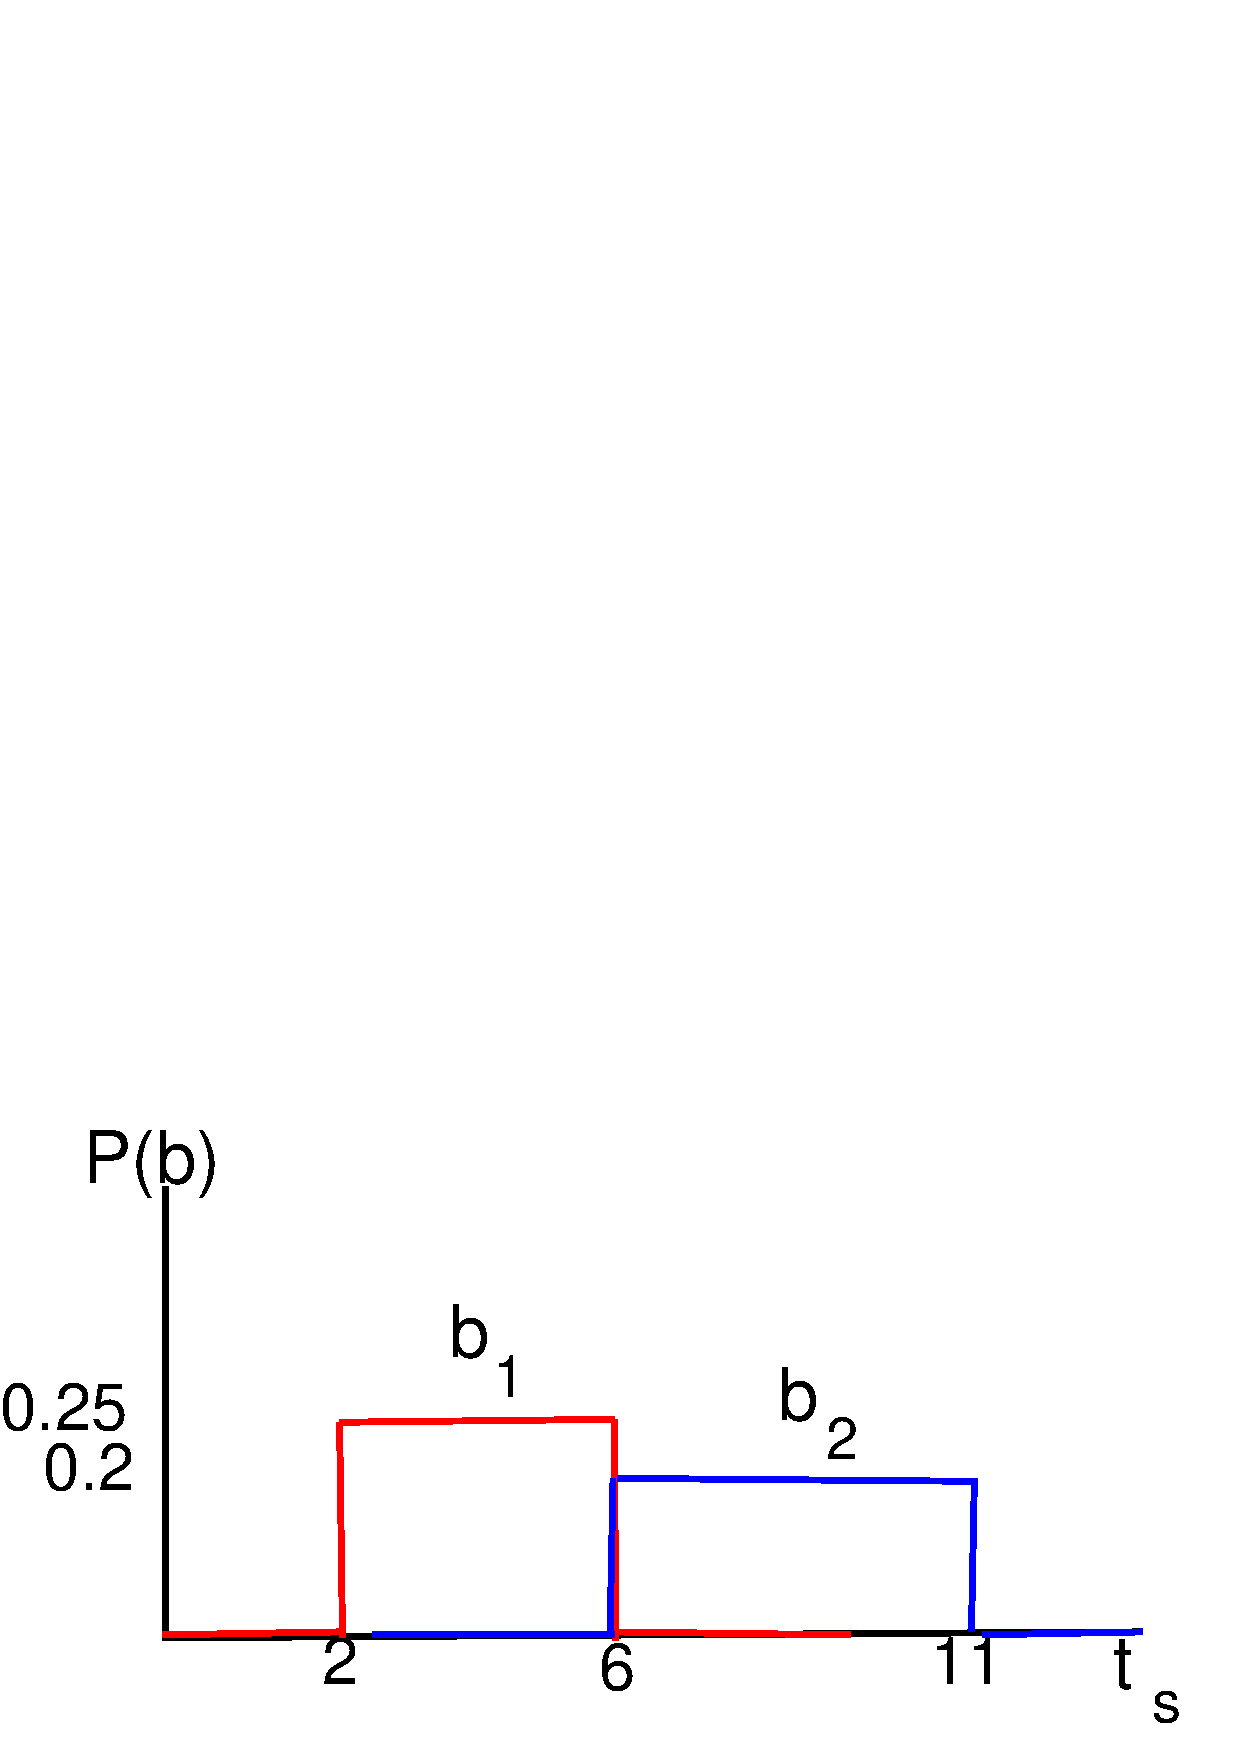
\includegraphics[width=0.41\textwidth]{pics/beliefs.pdf}
\hspace{-12mm}
\includegraphics[width=0.42\textwidth]{pics/delta1.pdf}
\hspace{-12mm}
\includegraphics[width=0.42\textwidth]{pics/delta2.pdf}
\hspace{-17mm}
\vspace{-10mm}
\caption{\footnotesize 
{\it (left)} Beliefs $b_1,b_2$ for 1D \textsc{Power Plant} example; 
{\it (middle)} Observation dependent function for $b_1$ that partition the observation space into 2 regions with different probabilities $P(z_i)$ ; 
{\it (right)} 3 Relevant observation partitions and their probabilities for $b_2$.
}
\label{fig:timeSpace}
\vspace{-4mm}
\end{figure*}
%%%%%%%%%%%%%%%%%%%%%%%%%%%%%%%%%%%%%%%%%%%%%%%%%%%%%%%%%%%%%%%%%%%%%%%%%% 
The observation dependent $\delta$-functions divide the observation space into regions which can yield the optimal policy according to the belief state $b_1$. According to continuous observation space defined in \cite{pascal_ijcai05}, for a 1-dimensional observation space with two or more functions of the observation, we need to find the optimal boundaries or partitions of the space. In their work, numerical solutions are proposed to find the roots of any two observation dependent function. Here we use the symbolic power of the max-operator to find all the maximum boundary regions of two or more $\delta$-functions at the same time. For the two $\delta$-functions above the following partitions of the observation space is derived after taking their maximum in line 6--7: 
{\footnotesize
\vspace{-2mm}
\begin{align}
\mathrm{max} \Bigg(\delta_{1}(t_o),\delta_{2}(t_o)\Bigg) &= 
\begin{cases}
 z_1:(t_o<2 : -0.4*t_o +6.8) \\
z_2:(t_o>2 : 1.3*t_o +3.4)
\end{cases}
\nonumber
\end{align}
}
The two partitions define observation regions which we can now use in a similar fashion to a discrete observation set if only the probability of each of the two distinct observation partitions is found. If we integrate out the state and observation from the observation model and the belief state regardless of a particular $\alpha$-vector, it integrates to one: 
$\int_{xd_o}\int_{xd_s} P(xd_o|xd'_s,a)*P(xd'_s|xd_s,a)*P(s) = 1$
Thus we only need to multiply the indicators of each case partition as as in line 9 in this formula to obtain the probability of each partition such that it sums to one: 
$P(z_k) := \int_{xd_o}\int_{xd_s} P(xd_o|xd'_s,a)*P(xd'_s|xd_s,a)*b_i* \mathbb{I}[\phi_{z_k}] d_{xd_o} d_{xd_s}$
For our example the probabilities are defined as $P(z_1)=0.2$ and $P(z_2)=0.8$.
%{\footnotesize
%\begin{align}
%P(z_k)=
%\begin{cases}
% (t_o<2) &: 0.2 \\
%(2<t_o) &: 0.8\\
%\end{cases} 
%\nonumber
%\end{align}
%}

Hence we can now use the algorithms and methods of a discrete observation setting using the probabilities of the partitioned observation space in Monahan's algorithm. 
%Figure ~\ref{fig:obsPartition} shows the observation partitions obtained in the 1D problem instance for different horizons and their related probabilities. In a lyx file, needed?
Next we present some results for 2-Dimensional continuous observation spaces.

%%%%%%%%%%%%%%%%%%%%%%%%%%%%%%%%%%%%%%%%%%%%%%%%%%%%%%%%%%%%%%%%%%%%%%%%%%
%\begin{figure}[tbp!]
%\vspace{-2mm}
%\centering
%\includegraphics[width=0.42\textwidth]{pics/nodes.pdf}\\
%\vspace{-2mm}
%\includegraphics[width=0.42\textwidth]{pics/time.pdf}
%\vspace{-2mm}
%\caption{\footnotesize space 
%and time vs. horizon.
%}
%\label{fig:timeSpace}
%\vspace{-4mm}
%\end{figure}
%%%%%%%%%%%%%%%%%%%%%%%%%%%%%%%%%%%%%%%%%%%%%%%%%%%%%%%%%%%%%%%%%%%%%%%%%%

\section{Empirical Results}
%We evaluated our continuous POMDP solution using XADDs on the one-dimensional
%\textsc{Power Plant} example and another variant of this problem with two variables. \footnote{
%Full problem specifications and Java code to reproduce these experiments are currently 
%in Google Code; anonymity restrictions prevent us from providing this link in the submitted paper version.}
The 2-dimensional model description is provided below:
%%%%%%%%%%%%%%%%%%%%%%%%%%%%%%%%%%%%%%%%%%%%%%%%%%%%%%%%%%%%%%%%%%%%%%%%%%
\begin{figure*}[tbp!]
\vspace{-2mm}
\centering
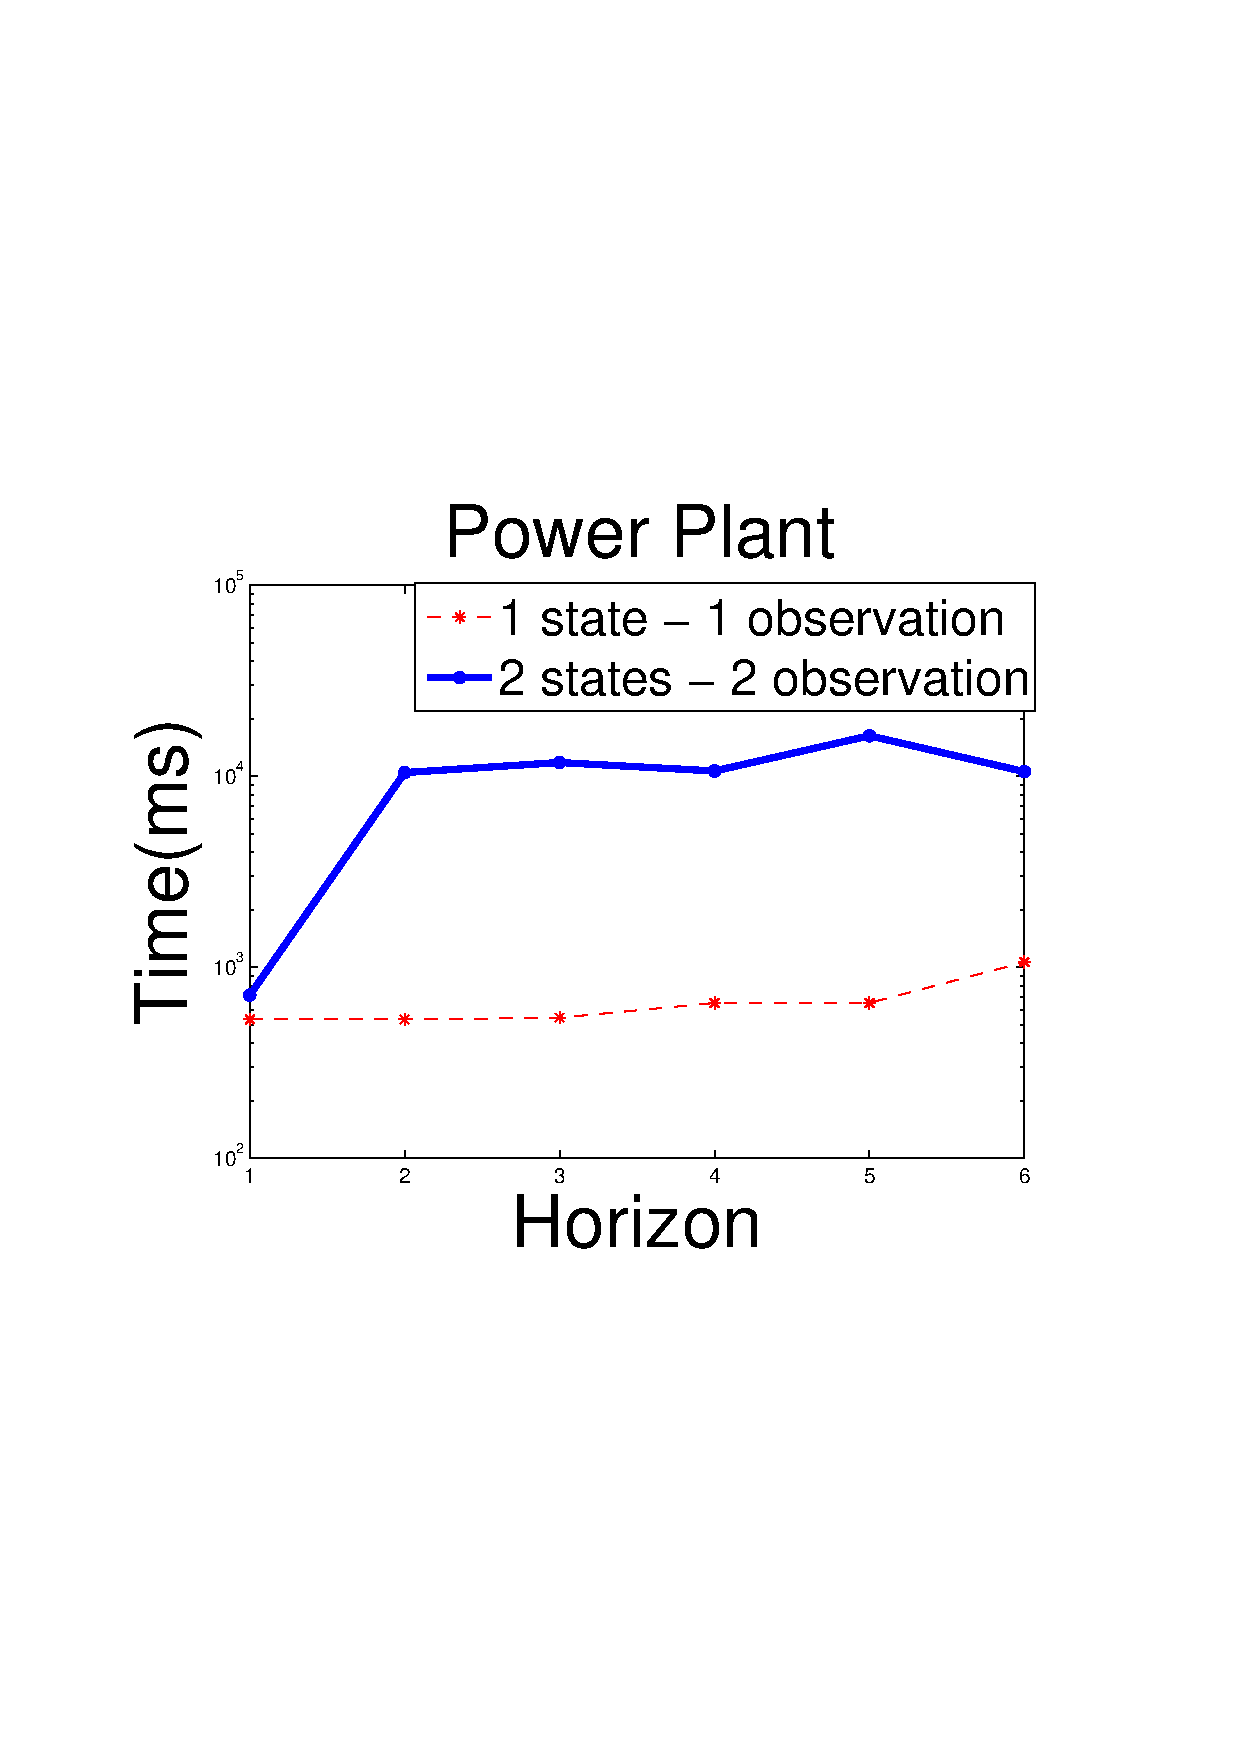
\includegraphics[width=0.3\textwidth]{pics/time2.pdf}
\includegraphics[width=0.3\textwidth]{pics/nodes2.pdf}
\includegraphics[width=0.3\textwidth]{pics/alpha-vectors2.pdf}
\vspace{-3mm}
\caption{\footnotesize 
{\it (left)} Space vs Horizon; 
{\it (middle)} Time vs Horizon; 
{\it (right)} Number of $\alpha$-vectors vs Horizon.
}
\label{fig:timeSpace}
\vspace{-4mm}
\end{figure*}
%%%%%%%%%%%%%%%%%%%%%%%%%%%%%%%%%%%%%%%%%%%%%%%%%%%%%%%%%%%%%%%%%%%%%%%%%% 

{\bf \textsc{2D-Power Plant}:} We consider the more complex model of the power plant similar to \cite{steam2} where the pressure inside the water tank must be controlled to avoid mixing water into the steam or explosion of the tank. We model the pressure variable $p$ as a partially observable variable from the observation readings of the pressure $po$. The two actions of increase and decrease are defined based on the change in both the temperature and the pressure. For the increase action we define: %the transition functions and the reward function is defined as below: 
{\footnotesize
\begin{align}
P(p_s'|\vec{p_s},inc)&= \delta\left[ p_s' - 
\begin{cases}
 (p+10> 20) &: 20 \\ 
\neg (p+10> 20) &: p_s + 10 \\
\end{cases}
\right]\nonumber
\hspace{5mm} 
P(t_s'|\vec{t_s},inc)= \delta\left[ t_s' - (t_s +10) \right]\nonumber
\end{align}
}
There is a high reward for staying withing the safe temperature and pressure range since it produces power, else depending on how safe it is to have values higher or lower than the safe range, penalty is defined.
{\footnotesize
\vspace{-4mm}
\begin{align}
R(t_s,p_s,inc) &= 
\begin{cases}
(5 \leq p_s \leq 15)\wedge (95 \leq t_s \leq 105)&:50\\
(5 \leq p_s \leq 15)\wedge (t_s \leq 95)&: -1\\
%(5 \leq p_s \leq 15)\wedge (t_s \geq 95)&: -3\\				
%(p_s \leq 5) &: -3\\						
(p_s \geq 15) &: -5\\ 
else &: -3
\end{cases}\nonumber
\end{align}
}
As for the decrease action, the transition functions reduce the temperature by 5 units and the pressure by 10 units as long as the pressure stays above zero. For the reward function, we assume that there is always a small penalty for decreasing the values because power can not be generated. 
For the observation model we consider two continuous uniform distributions such as the following:  
{\footnotesize
\begin{align}
P(t_o|t_s') = 
\begin{cases}
(t_s + 80<t_o<t_s+ 105) &: 0.4 \\
 \neg (t_s + 80<t_o<t_s+ 105) &: 0 \\
\end{cases}\nonumber
\hspace{5mm} 
P(p_o|p_s') = 
\begin{cases}
(p_s<p_o<p_s+10) &: 0.1 \\
 \neg(p_s<p_o<p_s+10) &: 0 \\
\end{cases}\nonumber
\end{align}
}
We define two rectangular uniform beliefs around the regions of rewarding, so that one needs to increase the values while the other should decrease them: $b_1: U[t_s;90,100]*U[p_s;0,10]$ and $b_2: U[t_s;90,130]*U[p_s;10,30]$
%\begin{align}
%b_1 = 
%\begin{cases}
%(p_o>p_s) \wedge (p_o<p_s+10) \wedge (t_o>t_s+ 90) \wedge (t_o<t_s+ 100)&: 0.01 \\
% \neg( (p_o>p_s) \wedge (p_o<p_s+10) \wedge (t_o>t_s+ 90) \wedge (t_o<t_s+ 100)) &: 0 \\
%\end{cases}\nonumber
%\end{align}
%\begin{align}
%b_2 = 
%\begin{cases}
%(p_o>p_s +10) \wedge (p_o<p_s+30) \wedge (t_o>t_s+ 90) \wedge (t_o<t_s+ 130)&: 0.00125 \\
% \neg((p_o>p_s +10) \wedge (p_o<p_s+30) \wedge (t_o>t_s+ 90) \wedge (t_o<t_s+ 130)) &: 0 
%\end{cases}\nonumber
%\end{align}
% I can draw this and the 1D belief
In Figure ~\ref{fig:timeSpace}, a time and space analysis of
the two versions of \textsc{Power Plant} have been performed for up to 6 horizons. %Comparing the two problem sizes demonstrates the effect of the number of state-observation variables in our algorithm. 
As the algorithm progresses, the time required to compute the probability of the partitions and finding the maximum $\alpha$-vector with respect to beliefs increases for both problem sizes and significantly more for the 2D version. %The stability in time is due to the fact that each stage almost takes the same time since it has converged quickly.%???
Increase in the problem size, increases the partition numbers on the observation space and this produces more $\alpha$-vectors which also effects the space required to perform the algorithm. The number of vectors stays the same for most horizons and they drop after convergence in the 2D problem instance. %The number of nodes in each iteration increases as more space is required to perform higher iterations.
This shows that although the 2D instance takes more time and space than the 1D instance, it still converges within reasonable resources.

In Figure ~\ref{fig:3D}  we present plots of the maximum $\alpha$-vectors of belief $b_1$ for different iterations of the 2D problem instance. %Each plot demonstrates the value of each vector as a function of the pressure and temperature. 
Starting with the first iteration, the value is highest for the reward range ($5<p<15 \wedge 95<t<105$) and -1 or less for other places. In the fifth iteration, the value function has partitioned into more pieces, showing how higher temperatures can increase the value without considering the effect of the pressure. In the last plot, horizon 6 has better tuned the value function so that higher temperatures and pressures increase the value of the maximum $\alpha$-vector and also within the reward range, finer grain partitions have been formed. %Also note that the policy depends on the initial belief and for these plots they were based on $b_1$ which was lower than the reward range. The first action would then mean it has performed an increase while the other iterations decrease and increase respectively.  
%%%%%%%%%%%%%%%%%%%%%%%%%%%%%%%%%%%%%%%%%%%%%%%%%%%%%%%%%%%%%%%%%%%%%%%%%%
% policy2, v2plot.pdf, v9plot
% annotation?
\begin{figure*}[tbp!]
\vspace{-2mm}
\centering
\includegraphics[width=0.31\textwidth]{pics/2d1.pdf}
\includegraphics[width=0.31\textwidth]{pics/2d9.pdf}
\includegraphics[width=0.31\textwidth]{pics/2d111.pdf}
\vspace{-3mm}
\caption{\footnotesize 
{\it (left)}Maximum $\alpha$-vector for $b_1$ in first iteration; 
{\it (middle)} $\alpha_{max}^5(b_1)$; 
{\it (right)} $\alpha_{max}^5(b_1)$.%V^6(p,t)
}
\label{fig:3D}
\vspace{-4mm}
\end{figure*}
%%%%%%%%%%%%%%%%%%%%%%%%%%%%%%%%%%%%%%%%%%%%%%%%%%%%%%%%%%%%%%%%%%%%%%%%%% 

\section{Conclusion} 
%This work has used the concept of continuous states and the SDP solution to MDPs from ~\cite{sanner_uai11} and continuous observations from the work of \cite{pascal_ijcai05}. It is exclusive in the sense that it brings together the continuous state and observation POMDPs using a symbolic approach. 
%In many applications of the POMDP framework, the state and observation space have been considered as discrete values such as ~\cite{steam2} here we avoid this general simplification and work with the real values from sensors.
%%sampling, monte carlo, particle filter, gaussians, perseus, pergeus
%
%There has been prior work on approximate solutions to POMDPs with large or continuous state spaces ~\cite{Thrun99h}, ~\cite{Perseus} and some has been extended to the continuous observation setting using methods such as sampling ~\cite{Perseus_cont}.
%In most approximate continuous state POMDP work, continuous or large discrete actions has been used. Thus we can extend the current work using \cite{zamani_aaai12} to contain continuous actions and provide exact or approximate solutions. 
%
%%\section{Conclusion}
We presented the first exact solution to continuous states and observations in a DC-POMDP framework. Transitions and reward functions are defined as piecewise linear functions of the continuous states. Continuous observations require definition of explicit partitions based on the observation model and the belief state of the agent. The key contribution is to define the partitions on the observation space and derive the related probabilities using symbolic integration and maximization. We extend the application to more than one state-observation setting and present the results.  
 
%\subsubsection*{References} 
\bibliography{dcpomdp}
\bibliographystyle{plain}

\end{document}
